\underline{Model wpływu społecznego}\newline
Wprowadźmy następujące oznaczenia:
\begin{itemize}
	\item $ \sigma_i(t) $ - opinia $ i $-tego agenta, $ \sigma_i(t) \in \{-1, 1\} $
	\item $ I_i(t) $ - "pole społeczne" oddziałujące na $ i $-tego agenta (wynika ono z obecności innych agentów)
	\item $ S_i $ - możliwość popierania (podtrzymania opinii) i-tego agenta, $ S_i $ > 0
	\item $ \prod_i $ - umiejętność perwazji (przekonania do swojej opinii) $ i $-tego agenta, $ \prod_i $ > 0
	\item $ d_{ij} $ - odległość społeczna między $ i $-tym, a $ j $-tym agentem
	\item $ g(d_{ij}) $ - osłabienie oddziaływań pomiędzy agentami w zależności od ich odległości społecznej, zazwyczaj $ g(d_{ij}) = A \cdot d_{ij}^{\alpha} $, $A, \alpha > 0 $, $ g(d_{ij}) = g(0) = \dfrac{1}{\beta} $
	\item $ \beta $ - parametr przekonania do własnej opinii
\end{itemize}

Poniższy wzór opisuje dynamikę modelu:\newline
$ \sigma_i(t + \Delta t) = - sign[\sigma_i (t) I_i(t)] $, gdzie:\newline

$ I_i(t) = \sum_j \dfrac{-[\sigma_i(t)\sigma_j(t) + 1]S_j}{2g(d_{ij})} + \sum_j \dfrac{[\sigma_i(t)\sigma_j(t) - 1]\prod_j}{2g(d_{ij})} + \eta_i(t) $, gdzie:\newline

$ \eta_i(t) $ – czynnik temperaturowy (szum losowy) o właściwościach $ <\eta_i(t)> = 0 $,  $ <(\eta_i(t))^2> = T $.
Kiedy stworzymy dwie sieci (grupy) agentów, o różnych opiniach, w których $ T_1 > T_2 $ i porównamy je ze sobą to grupa o wyższej temperaturze jest bardziej podatna na zmianę opinii.

Wybrany agent zmieni swoja opinię na przeciwną, kiedy pole społeczne
przyjmie wartość dodatnią. Innymi słowy, jego opinia ulegnie zmianie, wtedy gdy presja otoczenia będzie wystarczająco duża.

\underline{Model silnego lidera}\newline
Zakładamy poniższe wartości parametrów:\newline
$ \forall i \neq L, S_i = \prod_i = 1, S_L = \prod_L \gg 1 $

Otrzymujemy poniższe równanie na "pole społeczne":\newline
$ I_i(t) = \sum_{i\neq L} \dfrac{-\sigma_i(t)\sigma_j(t)}{g(d_{ij})} - \dfrac{\sigma_i(t)\sigma_L(t)}{g(d_{iL})}S_L $

\begin{figure} [H]
	\centering
	\begin{subfigure}{.99\textwidth}
		\centering
		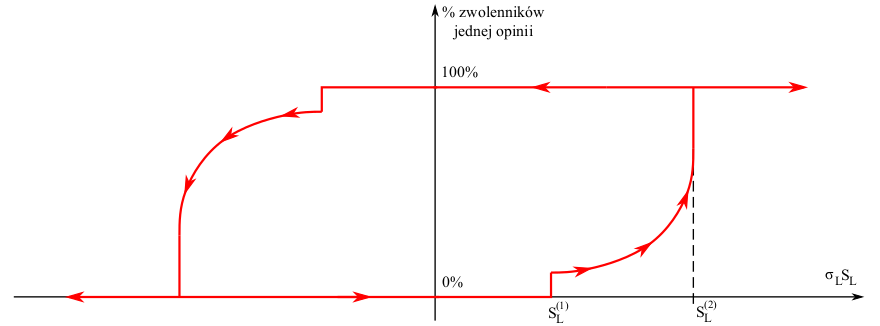
\includegraphics[width=1.0\linewidth]{EDMIIssues/Figures/lider.png}
	\end{subfigure}
	\caption{Proces zwolenników jednej opinii w funkcji iloczynu siły perswazji lidera i jego opinii. Wykres ten przypomina pętle histerezy, obserwowaną m.in. w zjawiskach magnetycznych.}
	\label{lider}
\end{figure}

Dla modelu silnego lidera istnieje wartość krytyczna $ S_L $ po której wszyscy agenci w grupie przyjmują wspólną opinię (rys.~\ref{lider}).

\underline{Model votera (wyborcy)} - agenci umiejscowieni są w sieci, w której możemy wyróżnić najbliższe sąsiędztwo każdego z nich. Każdy agent posiada pewną opinię (stan) $ s_i(t) \in {-1, 1} $. Dynamika przebiega w sposób następujący sposób:
\begin{itemize}
	\item Wylosuj agenta $ i $,
	\item Wylosuj agenta $ j $ będącego sąsiadem agenta $ i $,
	\item Agent $ i $ przyjmuję opinię agenta $ j $: $ s_i(t+\Delta t) = s_j(t) $.
\end{itemize}

W przypadku kiedy sieć jest prosta (tzn. każdy agent ma jednakową liczbę sąsiadów) wtedy układ osiąga stan równowagi $ <s_i> = const $. Innymi słowy liczba aktywnych interfejsów $ \rho (t) $ (połączeń agentów o przeciwnych opiniach) zanika w czasie.

Model votera można wzbogacić o koewolucję (ewoluuj ą zarówno stany węzłów jak i topologia samej
sieci). Dynamika koewolucji:
\begin{itemize}
	\item Z prawdopodobieństwem $ 1 - p $ agent $ i $ przyjmuje stan agenta $ j $, tak jak w zwykłym modelu votera,
	\item z prawdopodobieństwem $ p $ agent $ i $ zrywa połączenie z agentem $ j $ i nawiązuje połączenie z losowym agentem, który nie jest jego sąsiadem i posiada taką samą opinie.
\end{itemize}

Załóżmy, że po bardzo długim czasie ($ t \to \infty $) średnia liczba linków aktywnych wynosi $ \rho_s = const. $ Istnieje wtedy pewne prawdopodobieństwo krytyczne $ p = p_c $, dla którego $ \rho_s = 0 $ (rys.~\ref{density}).

\begin{figure} [H]
	\centering
	\begin{subfigure}{.7\textwidth}
		\centering
		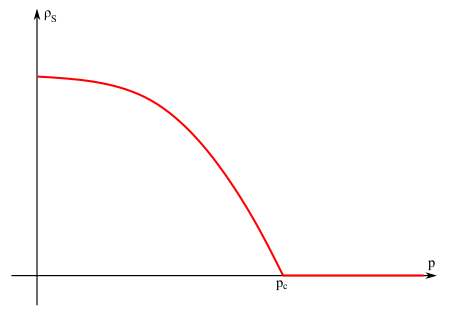
\includegraphics[width=1.0\linewidth]{EDMIIssues/Figures/density.png}
	\end{subfigure}
	\caption{Wykres zależności średniej gęstości aktywnych połączeń po bardzo długim czasie w funkcji prawdopodobieństwa $ p $.}
	\label{density}
\end{figure}

\underline{Model Axelroda} - każdemu agentowi przypisujemy wektor cech (np. wyznawana religia, poglądy polityczne) o długości $ F $, z których każda może posiadać $ q $ wariantów. Przebieg dynamiki:
\begin{itemize}
	\item wybieramy losowo agenta $ i $,
	\item wybieramy losowo agenta $ j $ z najbliższego sąsiedztwa agenta $ i $
	\item obliczamy liczbę wspólnych cech agentów $ i, j$:\newline
	$ l(i, j) = \sum_{f=1}^F \delta_{\sigma_{i,f}\sigma_{j,f}} $, gdzie $ \sigma_{i,f} $ - wariant cechy $ f $, agenta $ i $
	\item Spośród wszystkich cech, takich, że $ \sigma_{i,f} \neq \sigma_{j,f} $ wybieramy cechę $ k $ i zmieniamy opinię agenta $ i $: $\sigma_{i,k}(t+\Delta t) = \sigma_{j,k}(t) $ z prawdopodobieństwem $ p = \dfrac{l(i,j)}{F} $
\end{itemize}

\underline{Model większościowy} - zawiera $ N $ agentów, z których każdy ma opinię $ \pm 1 $. W dowolnej chwili czasu wybieramy $ m $ połączonych ze sobą agentów (zwykle losuje się jednego agenta oraz jego $ m - 1 $ różnych sąsiadów). Każdy agent z tak wylosowanej grupy przyjmuję opinię większości. Prawdopodobieństwo wylosowania agenta z opinią +1:\newline
$ a(t) = \dfrac{N_a(t)}{N} $, gdzie $ N_a(t) $ - liczba zwolenników opini +1 w chwili $ t $.

W najprostszym przypadku zakładamy, że wszyscy agenci są połączeni oraz $ m = 3 $. Wtedy:\newline
$ N_a(t+\Delta t) = N_a(t) + a(t)^2\cdot [1-a(t)] \cdot (+1) + a(t) \cdot [1-a(t)]^2 \cdot (-1) $,\newline
$ a(t + \Delta t) - a(t) = \dfrac{1}{N}a(t)[1-a(t)][2a(t) - 1] $.\newline
Jeśli za $ \Delta t $ przyjmiemy $ N $ wtedy otrzymamy poniższe równanie różniczkowe:\newline
$ \dot{a} = a(t + \Delta t) - a(t) = a(1-a)(2a - 1) = f(a) $\newline
Punkty stałe (miejsca zerowe funckji $ f(a) $) tego dynamicznego układu:\newline
$ a_- = 0, a_0 = 0.5, a_+ = 1 $
Stabilność otrzymancyh trzech punktów stałych badamy obliczając wykładnik Liapunowa $ \lambda (a) $ równy pochodnej $ f'(a) = -6a^2 +6a - 1 $ w tych punktach: \newline
$ \lambda(a_-) = -1 < 0 $ - punkt stabilny,\newline
$ \lambda(a_+) = -1 < 0 $ - punkt stabilny,\newline
$ \lambda(a_0) = 1/2 > 0 $ - punkt niestabilny.